Dans le cadre d'une liaison écoles-collège, une professeure d'EPS et une professeure des écoles organisent une course à vélo dont le parcours est composé de quatre tronçons en ligne droite.

La figure ci-dessous représente le parcours et n'est pas à l'échelle. Les élèves partent du point $A$ et tournent dans le sens des aiguilles d'une montre. Les dimensions sont les suivantes :
$$
AB=960~\text{m}, BC=1,05~\text{km}, CD=780~\text{m} \text{ et } AD=660~\text{m}.
$$

\begin{center}
	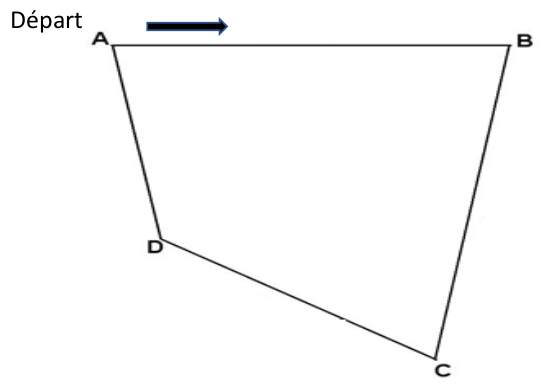
\includegraphics[width=.5\textwidth]{./images/2022-g2-ex2-img1.png}
\end{center}

\begin{enumerate}
  \item Montrer que le parcours a pour longueur $3~450~\text{m}$.

  \item Durant l'épreuve, Léo a réalisé, en 48 minutes, 2 tours complets et un tiers de tour du parcours.
	\begin{enumerate}
		\item Déterminer la distance parcourue par Léo.
		\item Donner la vitesse moyenne de Léo en $\text{km/h}$.
		\item En gardant la même vitesse moyenne, Léo aura-t-il parcouru $15~\text{km}$ en moins d'une heure et demie?Justifier.
	\end{enumerate}
  \item Une épreuve en relais est ensuite proposée. Tara parcourt les distances $AB$ et $BC$ à une vitesse moyenne de $10~\text{km/h}$ et Kevin parcourt les distances $CD$ et $DA$ à une vitesse moyenne de $6~\text{km/h}$.

Quelle est la vitesse moyenne de ce binôme sur l'ensemble du parcours ? Justifier.

  \item 
	\begin{enumerate}
	\item La diagonale [BD] mesure 1,05 km. Représenter le parcours à l'échelle $\dfrac{1}{20~000}$.
	\item Amina a roulé à vélo pendant 25 minutes à une vitesse moyenne de $11,5~\text{km/h}$.
	
	Placer sur la figure tracée à la question \textbf{4.a.} le point $S$ à l'endroit où se trouve Amina au bout de sa course. Justifier.
	\end{enumerate}
\end{enumerate}